\subsection{Selekcja}

\subsubsection{Kod źródłowy}


\subsubsection{Wyniki badań}


\begin{figure}[]
	\centering
	\hspace*{-0.8in}
	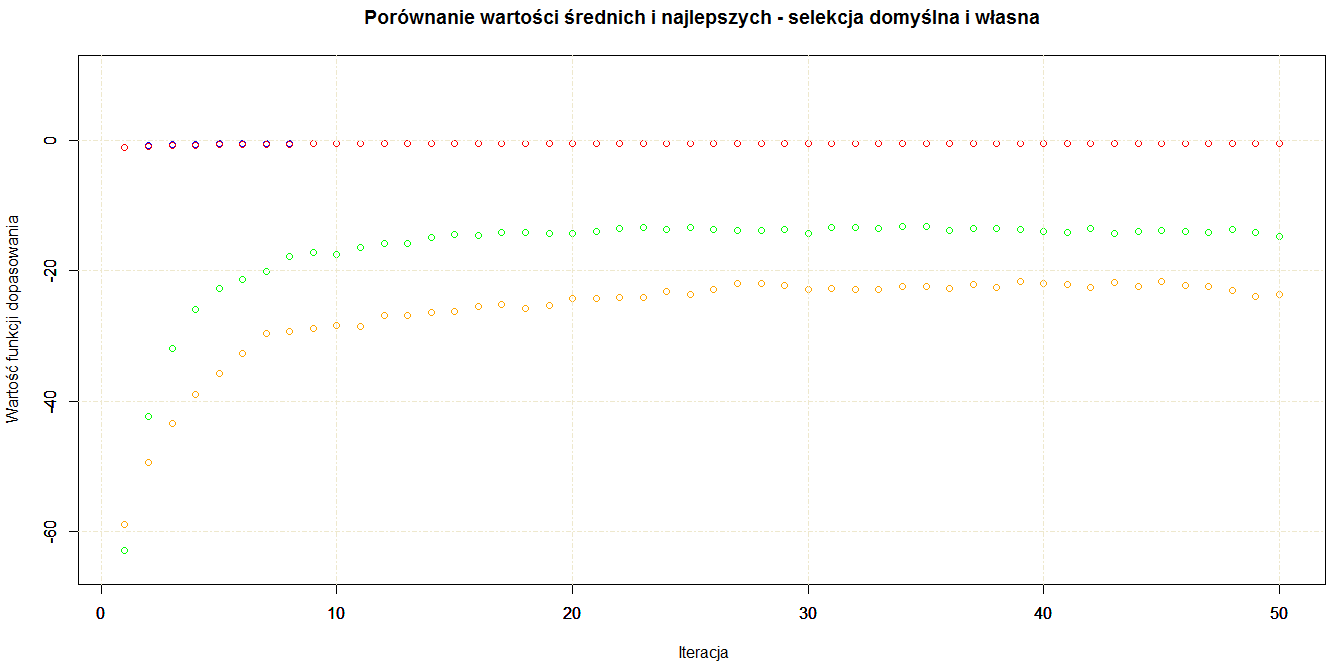
\includegraphics[scale = 0.5]{sel_1}
	\caption{Wykres przy 1 osobniku elitarnym}  
	\label{rys:sel_1} 
\end{figure}

\begin{figure}[H]
	\centering
	\hspace*{-0.8in}
	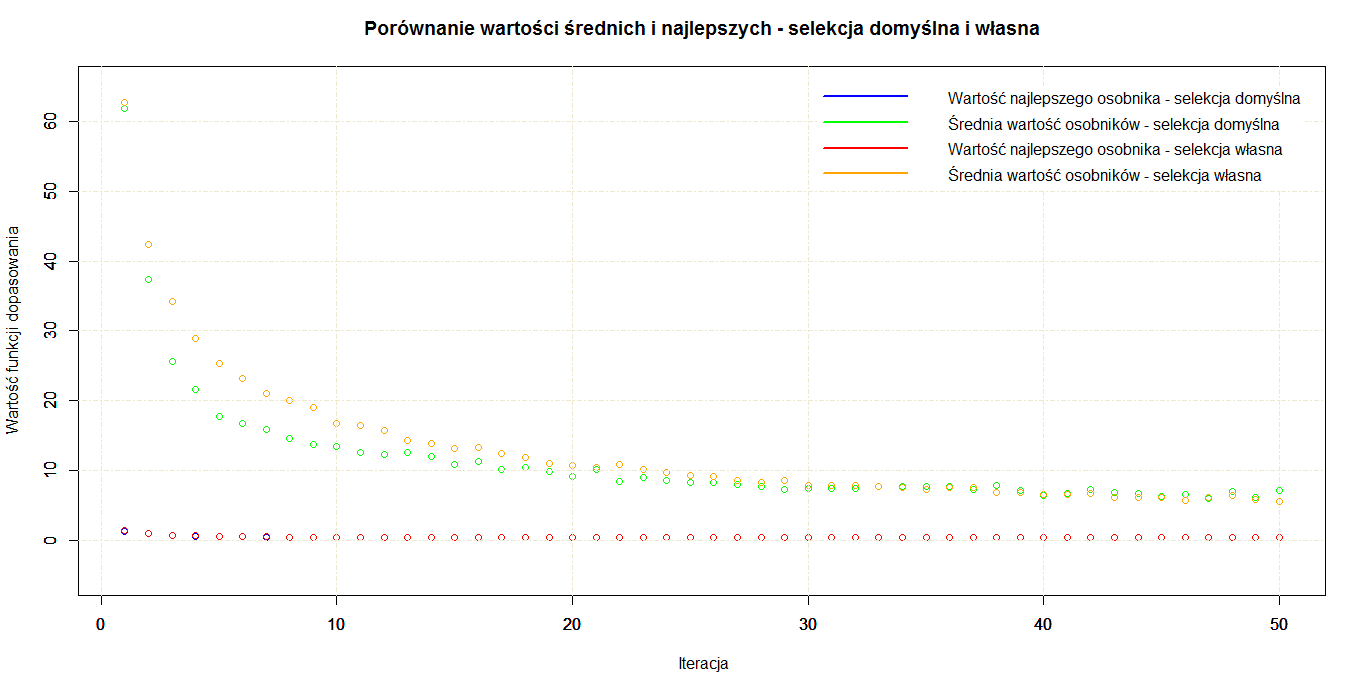
\includegraphics[scale = 0.5]{sel_6}
	\caption{Wykres przy 6 osobnikach elitarnych}  
	\label{rys:sel_6} 
\end{figure}

\begin{figure}[H]
	\centering
	\hspace*{-0.8in}
	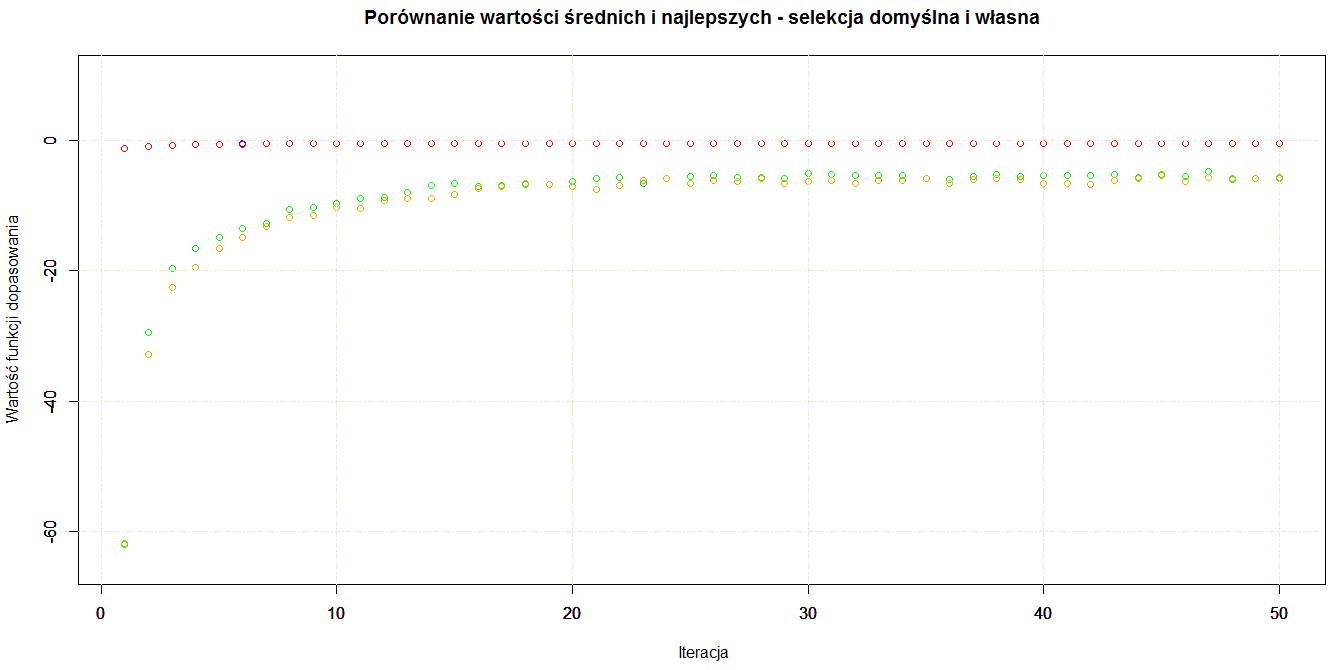
\includegraphics[scale = 0.5]{sel_20}
	\caption{Wykres przy 20 osobnikach elitarnych}  
	\label{rys:sel_20} 
\end{figure}

\begin{figure}[H]
	\centering
	\hspace*{-0.8in}
	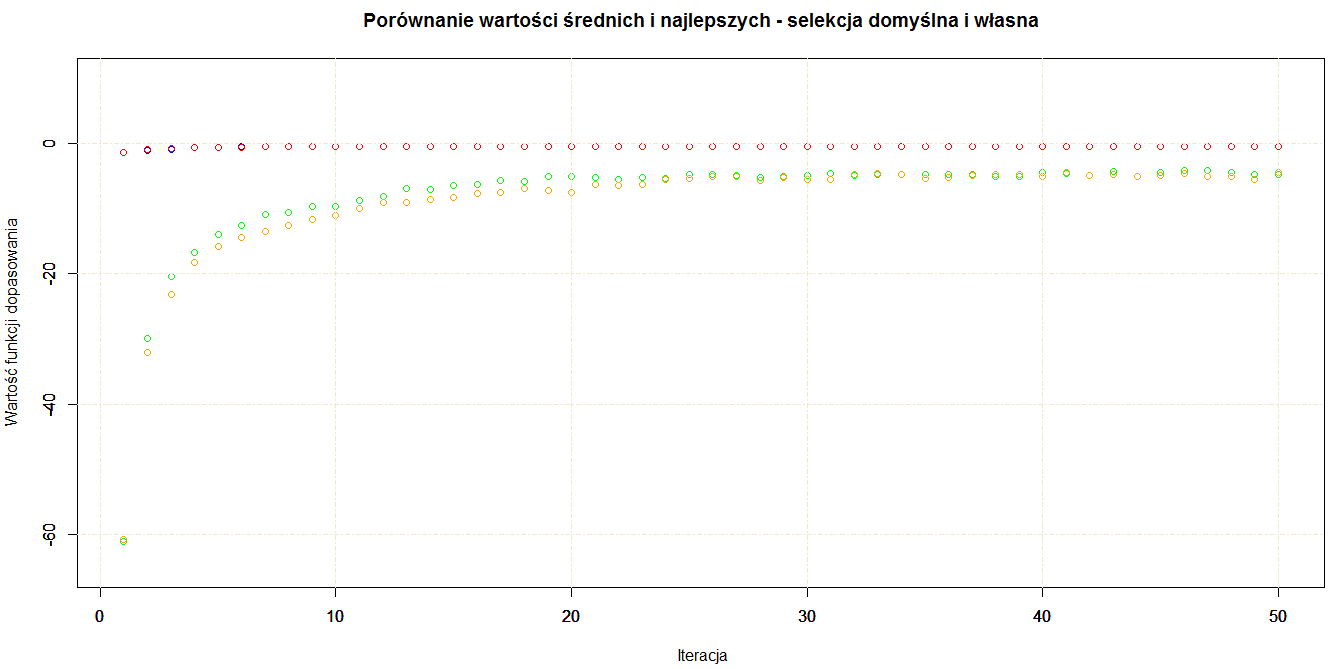
\includegraphics[scale = 0.5]{sel_50}
	\caption{Wykres przy 50 osobnikach elitarnych}  
	\label{rys:sel_50} 
\end{figure}

\subsubsection{Wnioski}

\begin{table}[!h]
	\centering
	\caption{Wartości średnie i najlepsze osobnika dla domyślnej i własnej funkcji selekcji}
	\label{sel_porownanie}
	\begin{tabular}{|c|c|c|c|c|}
		\hline
		\textbf{Selekcja} & \multicolumn{2}{c}{\textbf{Selekcja domyślna}}  & \multicolumn{2}{|c|}{\textbf{Selekcja własna}} \\ \cline{2-5}
		\textbf{elitarna} & Wartość średnia & Najlepszy wynik & Wartość średnia & Najlepszy wynik \\ \hline
		
		1  & 13.660880  & 0.405495 & 22.860800 & 0.414707 \\
		6  & 7.106856 & 0.400895 & 5.544652 & 0.397909 \\
		20 & 5.847374 & 0.397888 & 5.678752 & 0.397977 \\
		50 & 5.42606 & 0.397903 & 4.833812 & 0.397888  \\ \hline      
	\end{tabular}
\end{table}